\usetikzlibrary{arrows.meta}
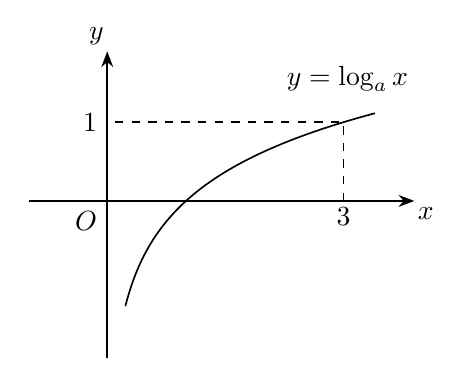
\begin{tikzpicture}[x=1cm,y=1cm,line width=.6pt,>=Stealth,font=\normalsize]
\draw[->] (-1.00,0) -- (3.90,0) node[below right,inner sep=0pt,xshift=1pt,yshift=-2pt] {$x$};
\draw[->] (0,-2.00) -- (0,1.90) node[above left,inner sep=0pt,xshift=-1pt,yshift=2pt] {$y$};
\draw[dashed] (3,0) -- (3,1) -- (0,1);
\draw[domain=0.23:3.40,samples=160] plot (\x,{ln(\x)/ln(3)});
\node[anchor=north east,inner sep=0pt] at (-0.12,-0.12) {$O$};
\node[anchor=east,inner sep=0pt] at (-0.12,1) {$1$};
\node[below,inner sep=0pt,yshift=-2pt] at (3,0) {$3$};
\node[inner sep=0pt] at (3.05,1.55) {$y=\log_a x$};
\end{tikzpicture}
